\subsection{Supersafety $\rightarrow$ Perfect Timeliness}\label{sec:backward-reduction}

We now construct a perfectly timely protocol $\Pi^*$
using a black-box reduction from a supersafe, and live($u$) protocol $\Pi$.
Each honest party $P$, executing the $\Pi^*$ protocol, runs a
full node of protocol $\Pi$.
The main idea is that, even though $\Pi$ is not a temporal ledger,
since it is supersafe, we can simply
ascribe to each new transaction the round at which it first appeared on our ledger
without loss of safety.
% The ledger of party $P$ for protocol $\Pi$ and $\Pi^*$ is denoted as $\Ledger[][P][r]$ and
% $\Ledger[*][P][r]$ respectively.
% To construct temporal ledger $\Ledger[*][][r]$,
% new transactions appearing in
% $\Ledger[][][r]$ are appended to $\Ledger[*][][r - 1]$ with recorded round $r$.
This reduction is illustrated in Figure~\ref{fig:backward-reduction}
and Algorithm~\ref{alg:backward-reduction}.

\import{./}{algorithms/algorithm-backward-reduction.tex}

\begin{figure}
  \centering
  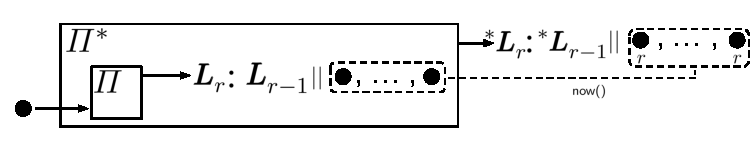
\includegraphics[width=0.9\columnwidth,keepaspectratio]{figures/backward-reduction.pdf}
  \caption{The reduction from Supersafety
    (the $\Pi$ protocol) to Perfect Timeliness (the $\Pi^*$ protocol).
    New transactions of $\Ledger[][][r]$ are included in
    $\Ledger[*][][r]$ with recorded round $r$.
  }
 \label{fig:backward-reduction}
\end{figure}

%We now prove that protocol $\Pi^*$ is perfectly timely.

\begin{theorem}[Supersafety to Perfect Timeliness] \label{thm:backward-reduction}
  An execution of $\Pi^*$ is perfectly timely, supersafe, and live($u$), if the execution of
  $\Pi$ is supersafe and live($u$).
\end{theorem}
\begin{proof}
  Timeliness requirements (1) and (2) are directly satisfied.
  For (3) consider any honest party $P$ and any rounds $r_1 \leq r_2$.
  Only transactions with recorded round greater
  than $r_1$ appear in ledger $\Ledger[*][P][r_2]{[|\Ledger[*][P][r_1]|{:}]}$.
  Hence, $\Pi^*$ is timely with parameter $v = 0$.
  Supersafety and liveness($u$) follow from those of $\Pi$.
  \Qed
\end{proof}

\subsection{A Perfectly Timely, Supersafe Protocol with Clients}

The protocol of the last subsection is perfectly time and supersafe.
But how about late-joining clients?
When a client first boots, it obtains all past transactions
from $\Pi$.
However, since $\Pi$ is not temporal, the client does not see any recorded rounds
associated with the transactions. Additionally, since the recorded rounds depend
on past ledger append times, the client cannot deduce them on its own.

To enable client support, we make a small addition to the protocol:
Each node runs an \emph{additional} instance of the internal
ledger protocol $\Pi$
to facilitate the booting of clients.
We call $\Pi_1$ the first instance of $\Pi$
(which operates as before),
and $\Pi_2$ this new instance of $\Pi$.
The output ledger $\Ledger[*]$ of the nodes remains the same.
Since the online nodes have observed the rounds with which
transactions of $\Pi_1$ are reported, they record those
rounds on the second ledger $\Pi_2$ to help the client
recover them.
Let $\Ledger[1]$ and $\Ledger[2]$ be the output ledgers
of $\Pi_1$ and $\Pi_2$ respectively.
The instance $\Pi_2$ is used as follows:
In every round $r$, all honest nodes $P$ introduce a transaction
which contains the whole ledger $\Ledger[*][P][r]$ as its payload.
We parameterize $\Pi_2$ with the following transaction validity language:
Valid transactions contain any ledger $\hat \Ledger \preccurlyeq \Ledger[*][P][r]$.
The protocol is illustrated in Figure~\ref{fig:client-support}.

A late-joining client first synchronizes $\Pi_1$ and $\Pi_2$ with the rest
of the peers.
Due to safety, liveness and the validity rule of $\Pi_2$,
the client can read ledger $\Ledger[2]$ to find out the
recorded rounds of past transactions.
Eventually, all past transaction recorded rounds are included in $\Ledger[2]$
and the client can construct the correct temporal ledger $\Ledger[*]$.
At this point we say the client is fully booted and can continue
operating as a full online node without $\Pi_2$, i.e., it outputs the ledger $\Ledger[*]$.
From this point on, the client is perfectly timely and supersafe.

\begin{figure}
  \centering
  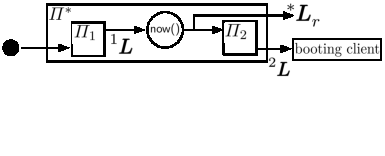
\includegraphics[width=0.7\columnwidth,keepaspectratio]{figures/perfectly-timely-clients.pdf}
  \caption{Client support for the perfectly timely and supersafe protocol $\Pi*$.
  }
 \label{fig:client-support}
\end{figure}

Lastly, to make this protocol efficient, we observe that the payload of
$\Pi_2$ transactions does not need to include whole ledgers, but can simply
include only the additional transactions that have since appeared on $\Ledger[1]$.
Lastly, the two instances of $\Pi$ can be combined into one by coloring
transactions appropriately: A normal transaction $\tx$, colored \emph{black}, enters into the
$\Pi^*$ protocol and is recorded on $\Pi$ as usual. When it stabilizes and its round
has been recorded by an online node, this node wraps the transaction $\tx$ into an
\emph{orange} transaction $\tx'$ containing as payload $\tx$ together with its recorded
round. The ledger output by $\Pi$ is split into black and orange parts. The black part
is reported as the output ledger of $\Pi^*$. The orange part is used to help clients boot,
and is ignored by a client after booting has finished. The validity language restrictions
only apply to the orange transactions. This final construction is illustrated in
Figure~\ref{fig:client-support-feedback}.

\begin{figure}
  \centering
  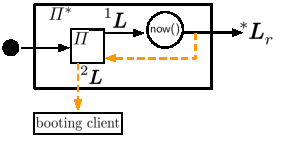
\includegraphics[width=0.55\columnwidth,keepaspectratio]{figures/perfectly-timely-clients-feedback.pdf}
  \caption{The client-supporting supersafe and perfectly timely protocol $\Pi^*$
           using only one instance of $\Pi$ for efficiency.
           Normal transactions and ledgers are shown in solid black lines;
           auxiliary transactions are shown in dashed
           orange lines.}
 \label{fig:client-support-feedback}
\end{figure}

